\chapter{\textbf{Proposed Navigation Filter Architecture}}
Tracking loops discussed in Chapter~3 are critically important to receivers as they adapt the replica signal to match the received signal data for proper decoding. However, traditional scalar loop filters assume a static noise bandwidth, regardless of receiver or satellite dynamics. If either platforms have unmodeled dynamics, these static bandwidths can permit too much noise into the navigation solution, or neglect some of the dynamics by filtering too much of the signal. One solution to this problem is implementing an adaptive Kalman filter to optimally select bandwidths~\cite{huangIntegratedAdaptiveKalman2019}. In the adaptive Kalman filter, the Kalman filter estimates the proper bandwidth based on discriminator residuals and modeled variances, but is agnostic to the dynamics of the receiver or the satellite dynamics. The addition of an adaptive Kalman filter is an improvement, but leaves a lot to be desired as each channel is still being tracked individually, resulting in low-powered channels having a high likelihood of being lost.

Another, more optimal, solution is to estimate the local replica signal from receiver and satellite dynamics at every integration period. This requires an updated estimate of the navigation solution at every integration period. This approach combines the adaptive bandwidth from~\cite{huangIntegratedAdaptiveKalman2019} along with knowledge of the receiver and satellite dynamics stemming from the navigation solution. This closed-loop approach is known as {vector tracking} and will be discussed in greater detail later on in this chapter. Specifically, the Vector Delay and Frequency Lock Loop (VDFLL) is the vector tracking implementation used in this thesis.

To build on vector tracking, this work proposes an addendum to the existing navigation filter architecture by adding a FVDM to predict the trajectory of flight vehicle. When coupling external propagation schemes to GPS measurements, there are three common regimes.

The simplest form is loosely-coupled, where receiver position and velocity measurements are coupled with the predicted states from the external sensor to provide an improved receiver state estimate (Figure~\ref{fig:LC}). The advantages of loose coupling is that the GPS receiver does not need to be modeled extensively; however, the noise provided by the receiver is not white, making the Kalman filter sub-optimal~\cite{lashleyPerformanceAnalysisVector2009}. Furthermore, a {loosely-coupled} architecture only works with at least 4 satellites are transmitting to the receiver {--} which is not always the case for GPS-challenged environments~\cite{grovesPrinciplesGNSSInertial2012}.

\begin{figure}[!ht]
    \centering
    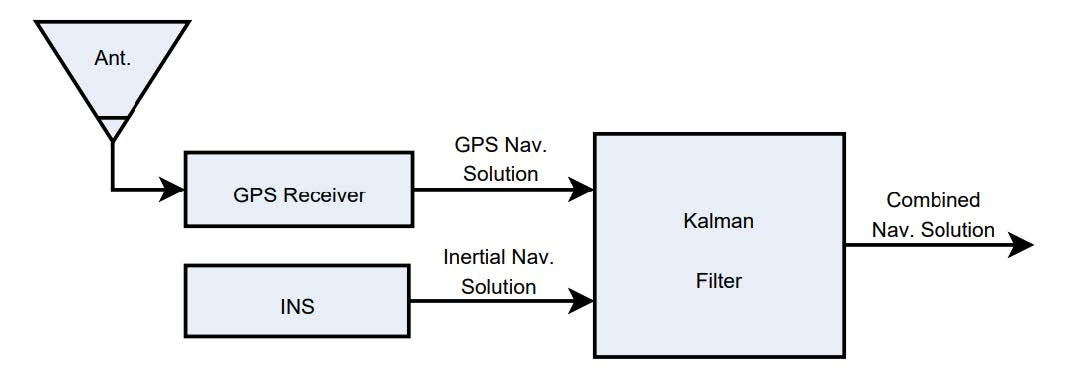
\includegraphics[width=\linewidth]{Figures/LC.jpg}
    \caption{Loosely-coupled architecture between GPS and INS systems~\cite{hammAnalysisSimulatedPerformance2005}.}\label{fig:LC}
\end{figure}

A more complicated coupling is {tightly-coupled}, where the navigation filter receives raw pseudorange and pseudorange rate measurements from the GPS receiver~\cite{kaplanUnderstandingGPSPrinciples2006} (Figure~\ref{fig:TC}). Because of this, tightly-coupled systems are still able to perform with less than 4 satellites, for a limited time. The draw back to tightly-coupled navigation architectures is the complexity of implementation. However, a working tightly-coupled system provides generous improvements over loosely-coupled frameworks, especially in GPS-challenged environments~\cite{grierPositionNavigationTiming}.

\begin{figure}[!ht]
    \centering
    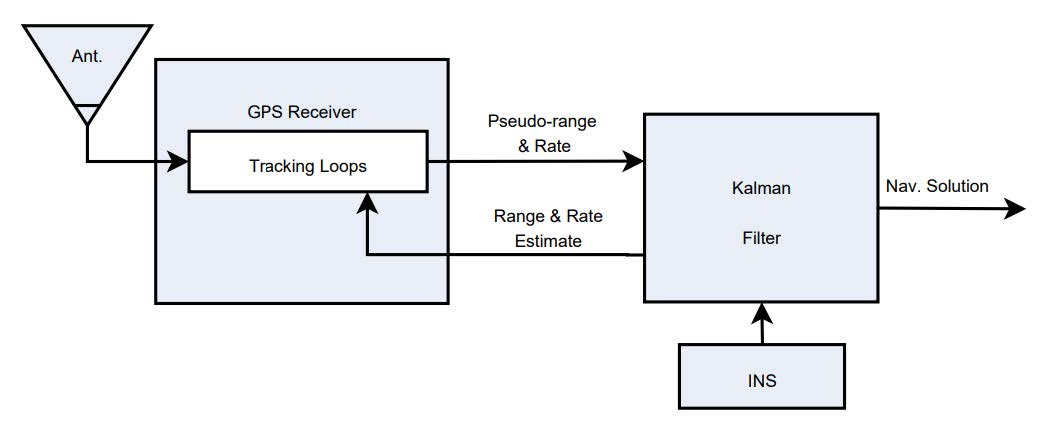
\includegraphics[width=\linewidth]{Figures/TC.jpg}
    \caption{Tightly-coupled architecture between GPS and INS systems~\cite{hammAnalysisSimulatedPerformance2005}.}\label{fig:TC}
\end{figure}

{Deeply-coupled}, or ultra-tight coupling, is the last of the common methods to couple external state predictions to GPS measurements. The downsides to deeply integrating an external sensor or vehicle dynamic model to GPS measurements is increased complexity and the reliance on the receiver to know its initial position {--} as is common with vector tracking. Generally, a deeply integrated system revolves around adapting the EKF that exists for a vector tracking architecture and appending the external dynamic model. This way, the GPS receiver and the added dynamic model are tied together at the most basic level. The benefits of a complete deeply-coupled system allow continued tracking of a degraded signal \(2-6\) dB higher than their scalar loop counter-parts~\cite{wattsGPSGLONASSL12019}. Furthermore, the addition of external dynamics allows better predictions of receiver pose due to the navigation filter acknowledging the dynamics of the collection platform. This is especially beneficial for high-dynamic vehicles such as hyper-velocity aircraft~\cite{pozzobonSupersonicGNSSAuthentication2014} or vehicles in GPS-challenged environments~\cite{martinGPSCarrierPhase2017}. For these benefits, a deep integration of the FVDM with GPS correlator-level measurements is the focus of this work.

\section{\textbf{Vector Delay and Frequency Lock Loop}}
Vector tracking first utilized a Vector Delay Lock Loop (VDLL) and was proposed by~\cite{e.m.coppsOptimalProcessingGPS1980}. In a VDLL\@, the EKF provides continuous estimates of the code frequency, updating the DLL, improving overall tracking performance. Later on,~\cite{bradfordparkinsonGlobalPositioningSystem1996}, explores tracking both code frequency and carrier frequency in an EKF, coined the VDFLL\@. This method showed great improvements over scalar tracking algorithms and moderate improvements over the VDLL\@. The VDFLL proves best when tracking weaker GNSS signals under high dynamic stress~\cite{lashleyPerformanceAnalysisVector2009}. Furthermore, recent analyses from~\cite{ziedanMultipathChannelEstimation2012} prove the VDFLL has improved resilience to multipath delay as well. A block diagram of the VDFLL is shown in Figure~\ref{fig:VDFLL}.

\begin{figure}[!ht]
    \centering
    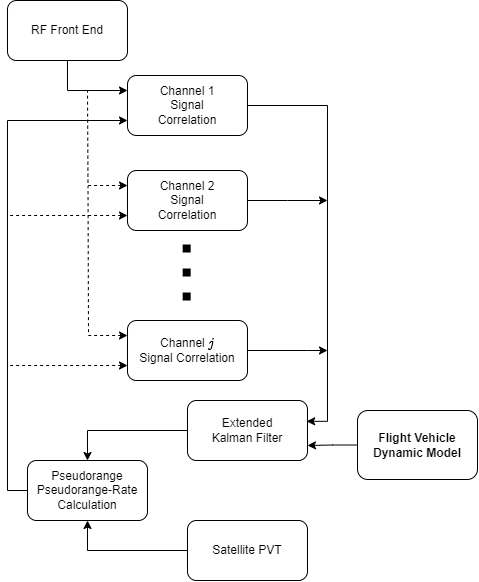
\includegraphics[width=0.45\linewidth]{Figures/VectorTracking.drawio.png}
    \caption{Block diagram of the VDFLL used in this work (Adapted from~\cite{grierPositionNavigationTiming}).}\label{fig:VDFLL}
\end{figure}

From Figure~\ref{fig:VDFLL}, the \textit{RF Front End} block refers to the discussion in Section~3.1. The signal correlation blocks represent Equation~\ref{eq:correlators} and also the the FLL and DLL discriminators specified in Equations~\ref{eq:FLLdisc} and~\ref{eq:DLLdisc}, respectively. The basic flow of the VDFLL requires the receiver to know its position and the positions of the satellites \textit{a priori}. Preferably, initial positions and satellite positions that are fed into the VDFLL are from processing the received signal for a length of time required to decode the navigation message using an open-loop architecture like the scalar tracking loops and WNLS discussed in Chapter 3. The measurement inputs of the EKF in Figure~\ref{fig:VDFLL} are residual pseudorange and pseudorange-rate errors in the form of discriminator outputs. The EKF uses the measurements from the current signal correlations to directly estimate the pose of the receiver. Using the ephemeris of the satellites and the corrected position estimates, new code phase and carrier frequency estimates are generated for the next integration period. To improve the estimated position from the EKF, the FVDM is used as the process model to propagate the non-linear motion of the aircraft in time. The next section covers the time update and measurement update within the EKF\@.

\section{\textbf{Deeply Coupled GPS and FVDM Navigation Filter}}
As stated previously, the VDFLL replaces the scalar DLLs and FLLs with a single EKF\@. This sections describes the design of the EKF for the proposed navigation filter. The EKF for this work represents a position-state filter where the state vector is defined by Equation~\ref{eq:stateVector}.

\begin{equation}\label{eq:stateVector}
    \mathbf{X} =
    \begin{bmatrix}
        \mathbf{X}_V & \mathbf{X}_{\omega} & \mathbf{X}_P & \mathbf{X}_{\psi} & \mathbf{X}_t \\
    \end{bmatrix}^T
\end{equation}

The essential elements for the state vector are sectioned into five terms.~\(\mathbf{X}_V\) (Equation~\ref{eq:velVector}) describes the velocity states of the aircraft from Earth to body with respect to the Local Navigation frame.

\begin{equation}\label{eq:velVector}
    \mathbf{X}_V =
    \begin{bmatrix}
        V_N & V_E & V_D \\
    \end{bmatrix}
\end{equation}

\(V_N\), \(V_E\), and \(V_D\) are the velocity components of the aircraft in the North, East, and Down directions, respectively. The angular rates (\(\mathbf{X}_{\omega}\)) are represented from inertial to body with respect to the body frame (Equation~\ref{eq:omegaVector}).

\begin{equation}\label{eq:omegaVector}
    \mathbf{X}_{\omega} =
    \begin{bmatrix}
        p_{ib}^b & q_{ib}^b & r_{ib}^b \\
    \end{bmatrix}
\end{equation}

\(p_{ib}^b\), \(q_{ib}^b\), and \(r_{ib}^b\) are the angular rates components of the aircraft about the body-fixed \(x\),\(y\), and \(z\) axes. The position estimates of the aircraft are from Earth to body with respect to the Local Navigation frame (Equation~\ref{eq:posVector}), similar to the velocity states.

\begin{equation}\label{eq:posVector}
    \mathbf{X}_P =
    \begin{bmatrix}
        \lambda_{eb}^n & L_{eb}^n & h_{eb}^n \\
    \end{bmatrix}
\end{equation}
\(\lambda_{eb}^n\), \(L_{eb}^n\), and \(h_{eb}^n\) are the latitude, longitude, and altitude of the aircraft with respect to the geodetic reference frame described in Chapter 2. Equation~\ref{eq:eulVector} represents the Euler angles of the aircraft, represented from body to the local navigation frame.

\begin{equation}\label{eq:eulVector}
    \mathbf{X}_{\psi} =
    \begin{bmatrix}
        \phi_{bn} & \theta_{bn} & \psi_{bn} \\
    \end{bmatrix}
\end{equation}

\(\phi_{bn}\), \(\theta_{bn}\), and \(\psi_{bn}\) are the roll, pitch, and yaw of the aircraft from the body to the navigation frame. Completing the state vector are the clock terms that represent estimates of the clock bias and clock drift of the receiver during flight (Equation~\ref{eq:clkVector}). The clock bias and clock drift are scaled by the speed of light (\(c\)) to give them units of meters and meters/second, respectively.

\begin{equation}\label{eq:clkVector}
    \mathbf{X}_t = \begin{bmatrix}
        c\delta t & c\delta\dot{t} \\
    \end{bmatrix}
\end{equation}

The dynamics of the aircraft are defined by

\begin{equation}\label{eq:eulerIntegration}
    \dot{\mathbf{X}} = F\left(\mathbf{X},f_{ib}^b,M_{ib}^b\right) + \mathbf{B}_{dyn}w_{dyn} + \mathbf{B}_{clk}w_{clk},
\end{equation}

where \(\mathbf{B}_{dyn}\) is the noise distribution matrix related to the dynamics (Equation~\ref{eq:Bdyn}).

\begin{equation}\label{eq:Bdyn}
    \mathbf{B}_{dyn} =
    \begin{bmatrix}
        \frac{\Delta t^2}{2}\mathbf{I}_{6,6} \\
        \Delta t\mathbf{I}_{6,6}             \\
        \mathbf{0}_{2,2}
    \end{bmatrix}_{14,8}
\end{equation}

\(w_{dyn}\) is the disturbance vector for the aircraft dynamics, as shown in Equation~\ref{eq:wDyn}. Equation~\ref{eq:Bdyn} shows that only the linear and angular accelerations are affected by the disturbances, but these errors trickle down into the kinematic equations for the position and Euler derivatives.

\begin{equation}\label{eq:wDyn}
    w_{dyn} = \begin{bmatrix}
        \sigma^2_{V_N} & \sigma^2_{V_E} & \sigma^2_{V_D} & \sigma^2_{p} & \sigma^2_{q} & \sigma^2_{r}
    \end{bmatrix}^T
\end{equation}
\(\sigma_{()}\) are additive white Gaussian noise that characterizes the stochastic motion of the aircraft for their respective, sub-scripted variables. The discretized process noise covariance matrix is a function of the time step and phase and frequency clock variances for the specified oscillator (Equation~\ref{eq:Qclk}).

\begin{equation}\label{eq:Qclk}
    \mathbf{Q}_{clk} =
    \begin{bmatrix}
        \sigma^2_b \Delta t + \sigma^2_{br}\Delta t^2 + \sigma^2_r \frac{\Delta t^3}{3} & \sigma^2_{br}\Delta t + \sigma^2_r \frac{\Delta t^2}{2}                      \\
        \sigma^2_{br} \Delta t + \sigma^2_r \frac{\Delta t^2}{2}                        & \frac{\sigma^2_r}{\Delta t} + \sigma^2_{br} + \frac{4}{3}\sigma^2_r \Delta t \\
    \end{bmatrix}
\end{equation}

\(\sigma^2_b\) is the variance of the noise process that drives the clock phase error in \(m^2/s\), \(\sigma^2_{r}\) is the noise variance that drives the clock frequency error in \(m^2/s^3\) and \(\sigma^2_{br}\) is the variance on the noise process that drives both the phase and frequency error in units of \(m^2/s^2\). For the receiver simulated in this work, an Oven Controlled Crystal Oscillator (OCXO) is used. More information on calculating the clock variance based on oscillator type can be found in~\cite{robertgroverbrownIntroductionRandomSignals2013}. The time step (\(\Delta t\)) is \(200\) Hz.

\(F\) is a set of non-linear equations that define the motion of the aircraft as a function of the current state in time (\(\mathbf{X}\)), the forces in the body frame (\(f_{ib}^b\)) and the moments about the body frame (\(M_{ib}^b\)). Calculation of the forces and moments were discussed in Chapter 2.

Calculations of the forces and moments and moments must be done in the body frame. Rotating all of the equations that build the total forces and moments acting onto the airframe into a global or local navigation reference frame would be cumbersome and introduce more complexity than necessary. However, because of the measurements generated from the correlators and discriminators are composed in the ECEF reference frame, the FVDM must be propagated with respect to the curvature of the Earth in a global frame. For this work, the equations of motion are rotated into the local navigation frame.

The state derivatives of the velocity components are defined in Equation~\ref{eq:acc}.

\begin{equation}\label{eq:acc}
    \begin{bmatrix}
        \dot{V_N} \\
        \dot{V_E} \\
        \dot{V_D} \\
    \end{bmatrix} =
    \mathbf{C}_{b}^{n}\frac{\mathbf{f}_{ib}^b}{m} - \left(2\mathbf{\Omega}_{ie}^n - \mathbf{\Omega}_{en}^n\right)
    \begin{bmatrix}
        V_N \\
        V_E \\
        V_D \\
    \end{bmatrix}
\end{equation}

The first term above represents the forces acting onto the airframe with respect to the body frame divided by the mass of aircraft, \(m\). For the purposes of this work, the mass of the aircraft is assumed constant. This specific force vector is rotated into the local navigation frame using \(\mathbf{C}_b^n\), defined in Equation~\ref{eq:ECEF2LNDCM}. The latter term in Equation~\ref{eq:acc} represents the rotation rate (Equation~\ref{eq:earthrotation}) of the Earth in skew-symmetric form and the transport rate (Equation~\ref{eq:transportrate}) in skew-symmetric form, both rotated into the local navigation frame and multiplied by the current velocity of the aircraft.

\begin{equation}\label{eq:earthrotation}
    \mathbf{\Omega}_{ie}^n =
    \omega_{ie}\begin{bmatrix}
        0                          & \sin\left(L_{eb}^n\right) & 0                          \\
        -\sin\left(L_{eb}^n\right) & 0                         & -\cos\left(L_{eb}^n\right) \\
        0                          & \cos\left(L_{eb}^n\right) & 0                          \\
    \end{bmatrix}
\end{equation}

Where \(\omega_{ie}\) is \(7.27\times10^{-5}\) radians/second.

\begin{equation}\label{eq:transportrate}
    \mathbf{\Omega}_{en}^n = \begin{bmatrix}
        0                & -\omega_{en,z}^n & -\omega_{en,y}^n \\
        \omega_{en,z}^n  & 0                & -\omega_{en,x}^n \\
        -\omega_{en,y}^n & \omega_{en,x}^n  & 0                \\
    \end{bmatrix}
\end{equation}

Where

\begin{equation}\label{eq:omega_en_n}
    \omega_{en}^n =
    \begin{bmatrix}
        V_E/(R_E + h_{eb}^n)               \\
        -V_N/(R_N + h_{eb}^n)              \\
        V_E\tan(L_{eb}^n)/(R_E + h_{eb}^n) \\
    \end{bmatrix}
\end{equation}

Above, \(R_E\) and \(R_N\) refer to the meridian and transverse radii of curvature as described in Equations~\ref{eq:meridiancurvature} and~\ref{eq:transversecurvature}, respectively.

The derivatives of the angular rates are defined as

\begin{equation}\label{eq:angacc}
    \begin{bmatrix}
        \dot{p}_{ib}^b \\
        \dot{q}_{ib}^b \\
        \dot{r}_{ib}^b \\
    \end{bmatrix} =
    {\mathbf{I}_{cg}^b}^{-1}\left[\mathbf{M}_{ib}^b -
        \begin{bmatrix}
            p \\
            q \\
            r \\
        \end{bmatrix} \times
        \left(\mathbf{I}_{cg}^b
        \begin{bmatrix}
            p \\
            q \\
            r \\
        \end{bmatrix}
        \right)
        \right],
\end{equation}
where \(\mathbf{I}_{cg}^b\) are the mass moments of inertia for the aircraft. For the purpose of this work, the aircraft is modelled symmetrically about each of the axes such that \(\mathbf{I}_{cg}^b\) only has terms along the diagonal.

The local navigation frame position derivatives are described by Equation~\ref{eq:posrate}.
\begin{equation}\label{eq:posrate}
    \begin{bmatrix}
        \dot{\lambda}_{eb}^n \\
        \dot{L}_{eb}^n       \\
        \dot{h}_{eb}^n       \\
    \end{bmatrix} =
    \begin{bmatrix}
        \frac{V_N}{R_N + h_{eb}^n}                                       \\
        \frac{V_E}{\left(R_E + h_{eb}^n\right)\cos\left(L_{eb}^n\right)} \\
        -V_D                                                             \\
    \end{bmatrix}\\
\end{equation}

The derivatives of the Euler angles are seen in Equation~\ref{eq:eulerRates}

\begin{equation}\label{eq:eulerRates}
    \begin{bmatrix}
        \dot{\phi}_{bn}   \\
        \dot{\theta}_{bn} \\
        \dot{\psi}_{bn}   \\
    \end{bmatrix} =
    \mathbf{C}_{\omega}
    \left(
    \begin{bmatrix}
            p \\
            q \\
            r \\
        \end{bmatrix} -
    \mathbf{C_n^b}\left(\omega_{ie}^n + \omega_{en}^n\right)
    \right)
\end{equation}

Calculation of the Euler rates is the difference between the current angular rates of the aircraft and the rotation of the Earth along with the transport rate, similar to the calculation of linear acceleration in Equation~\ref{eq:acc}. This difference is rotated by \(\mathbf{C}_{\omega}\) defined by Equation~\ref{eq:cOmega}.

\begin{equation}\label{eq:cOmega}
    \mathbf{C}_{\omega} =
    \begin{bmatrix}
        1 & \tan(\theta)\sin(\theta)    & \tan(\theta)\cos(\phi)      \\
        0 & \cos(\phi)                  & -\sin(\phi)                 \\
        0 & {\sin(\phi)}/{\cos(\theta)} & {\cos(\phi)}/{\cos(\theta)} \\
    \end{bmatrix}
\end{equation}

The last of the state derivatives are the clock terms. Both the clock drift and clock drift rate are scaled by the speed of light to give them units of \( m \, s^{-1}\) and \( m \, s^{-2}\).

\begin{equation}\label{eq:clkRates}
    \begin{bmatrix}
        c\delta \dot{t} \\
        c\delta\ddot{t} \\
    \end{bmatrix} =
    \begin{bmatrix}
        0 & 1 \\
        0 & 0 \\
    \end{bmatrix}
    \begin{bmatrix}
        c\delta {t}    \\
        c\delta\dot{t} \\
    \end{bmatrix}
\end{equation}

Once the state derivatives are calculated using the aforementioned equations of motions, they are integrated using Euler integrations to propagate the states forward in time. This provides the EKF with the predicted states for the current time step.

The other part of the prediction step in the EKF is the formation of the predicted covariance matrix \(\mathbf{P}^-_{k}\). This is defined by Equation~\ref{eq:pminus}.

\begin{equation}\label{eq:pminus}
    \mathbf{P}^-_{k} = \mathbf{\Phi}\mathbf{P}^-_{k-1} \mathbf{\Phi}^T + \mathbf{Q_d}
\end{equation}

\( \mathbf{\Phi}\) is defined as the state transition matrix. The state transition matrix is composed of \(\mathbf{X}\) and the relationship with each state derivative \( \dot{\mathbf{X}}\). This done by taking the Jacobian and is represented by Equation~\ref{eq:stateJacobian}.

\begin{equation}\label{eq:stateJacobian}
    \mathbf{J} = \frac{\partial \dot{\mathbf{X}}_{14,1}}{\partial \mathbf{X}_{14,1}}
\end{equation}

The evaluated Jacobian, \(\mathbf{J}\), is a square 14 row, 14 column matrix that varies as function of the forces and moments in time. These forces and moments can vary based on the disturbances and the controls inputs, so \(\mathbf{J}\) must be evaluated at every time step. Because of the complexity of the Jacobian, it is solved using the symbolic toolbox in MATLAB\@.

The state propagation is continuous, but \(\mathbf{\Phi}\) is discrete. This means that the Jacobian must be discretized. The discretization of the Jacobian from continuous to discrete is introduced by Equation~\ref{eq:Phi}

\begin{equation}\label{eq:Phi}
    \mathbf{\Phi} = \textrm{expm}(\mathbf{J}\Delta t)
\end{equation}

The discrete process noise covariance (\(\mathbf{Q}_d\)) encapsulates the disturbances onto the aircraft dynamics such that the EKF can better correct the states during the measurement update. To transform the process noise from continuous to discrete, Equation~\ref{eq:Qd} is used.

\begin{equation}\label{eq:Qd}
    \mathbf{Q_d} = \texttt{blkdiag}\left(\left[\mathbf{\Phi}\mathbf{B}_{dyn} \left(w_{dyn}w_{dyn}^T\right) \mathbf{B}_{dyn}^T \mathbf{\Phi}^T \Delta t\right], \mathbf{Q_{clk}}\right)
\end{equation}

Once the state and covariance prediction are calculated, the \textit{a priori} part of the EKF is complete. The EKF will continue to predict the state and covariance until measurements from the vector tracking receiver are available. The next subsection covers the measurement update of the EKF, correcting the predicted covariance and predicted states.

\subsection{\textbf{Update \textit{a posteriori}}}
The measurement update in the EKF utilizes the current predicted covariance and measurement covariance to optimally correct the predicted states and predicted covariance. Equation~\ref{eq:L} shows the calculation of the Kalman gain.

\begin{equation}\label{eq:L}
    \mathbf{K}_k = \mathbf{P}^-_k \mathbf{H}^T_k{\left(\mathbf{H}_k\mathbf{P}^-_k\mathbf{H}^T_k + \mathbf{R}_k\right)}^{-1}
\end{equation}

The Kalman gain, \(\mathbf{K}\), is a function of the observation matrix, \(\mathbf{H}\), measurement covariance matrix, \(\mathbf{R}\), and the predicted covariance, described previously. The observation matrix maps the residual pseudorange and pseudorange rates to the local navigation states. This is demonstrated by Equation~\ref{eq:H}.

\begin{equation}\label{eq:H}
    \mathbf{H}_k = \begin{bmatrix}
        \mathbf{u}^{n,j}_{1,3} & \mathbf{0}_{1,3} & \mathbf{0}_{1,3}            & \mathbf{0}_{1,3} & 0  & -1 \\
        \mathbf{0}_{1,3}       & \mathbf{0}_{1,3} & \mathbf{h}^j_{\rho p_{1,3}} & \mathbf{0}_{1,3} & -1 & 0  \\
    \end{bmatrix}_{2j,14}
\end{equation}

Using the predicted estimate of the receiver position Euler attitude, \(\mathbf{H}\) rotates the ECEF residuals to the local navigation frame. There are arrays of zeros where the measurements do not correlate to the corresponding states. The rotation of the unit vectors from ECEF to the local navigation frame is shown by Equation~\ref{eq:nav_u} and the rotation for the position measurements is given by Equation~\ref{eq:nav_h}.

\begin{equation}\label{eq:nav_u}
    \mathbf{u}^{n,j} = \mathbf{C}_e^n \mathbf{u}^{e,j}
\end{equation}

\begin{equation}\label{eq:nav_h}
    \mathbf{h}^j_{\rho p} =
    \begin{bmatrix}
        \left(R_N + h^n_{eb}\right)\mathbf{u}^{n,j}_N               \\
        \left(R_E + h_{eb}^n\right)\cos(L^n_{eb})\mathbf{u}^{n,j}_E \\
        -\mathbf{u}^{n,j}_D                                         \\
    \end{bmatrix}
\end{equation}

The measurement covariance matrix,~\(\mathbf{R}\), was described as the weighting matrix, \(\mathbf{W}\), in Chapter 3. The variances of the measurements are still calculated as a function of the carrier-to-noise ratio. Once the Kalman gain is calculated for the current time step, it can be used with the measurement vector, \(\Delta z\), to update the predicted state estimate (Equation~\ref{eq:deltaZ} and~\ref{eq:xplus}).

\begin{equation}\label{eq:deltaZ}
    \Delta z = \begin{bmatrix}
        \Delta\dot{\rho}^{\,1} & \Delta{\rho}^{\,1} & \hdots & \Delta\dot{\rho}^{\,j} & \Delta{\rho}^{\,j} \\
    \end{bmatrix}^T
\end{equation}

\begin{equation}\label{eq:xplus}
    \mathbf{X}_k^+ = \mathbf{X}^-_k + \mathbf{K}_k\Delta Z
\end{equation}

The last step in the measurement update is correcting the predicted covariance (Equation~\ref{eq:pplus}). The predicted covariance will drift based on the process noise covariance matrix and correcting the covariance by using the newly calculated Kalman gain will inform the filter of the confidence in the process model.

\begin{equation}\label{eq:pplus}
    \mathbf{P}^+_k = \left(\mathbf{I} - \mathbf{K}_k\mathbf{H}_k\right)\mathbf{P}^-_k
\end{equation}

After the measurement update of the EKF is complete, the estimated states and covariance matrices redefine the predicted state and covariances, closing the loop in the proposed navigation filter.

\section{\textbf{Conclusions}}
Vector tracking is a closed loop solution to estimating navigation states in a GPS receiver. The proposed navigation filter augments the existing VDFLL architecture by instantiating the FVDM as the process model in the EKF\@. This chapter covered the differences between scalar and vector tracking loops and expanded on the utilization of the FVDM to propagates the states of aircraft while also using correlator-level GPS measurements to correct the states and maintain channel lock for the duration of the simulations. This chapter provided a general overview of the VDFLL and covered the additions to the VDFLL architecture that did not exist before. For a more nuanced implementation of the VDFLL, the reader is asked to read the sources cited throughout the chapter for more information.